\section*{QUESTION \quesNo.}

\subsection*{Explanation/Theory}

\[
    x(t) = \cos\left(\frac{3\pi}{2} t\right) e^{-\frac{t^2}{2}}
\]

(a) Evaluate \(X(j\omega)\).

\begin{figure}[H]
    \centering
    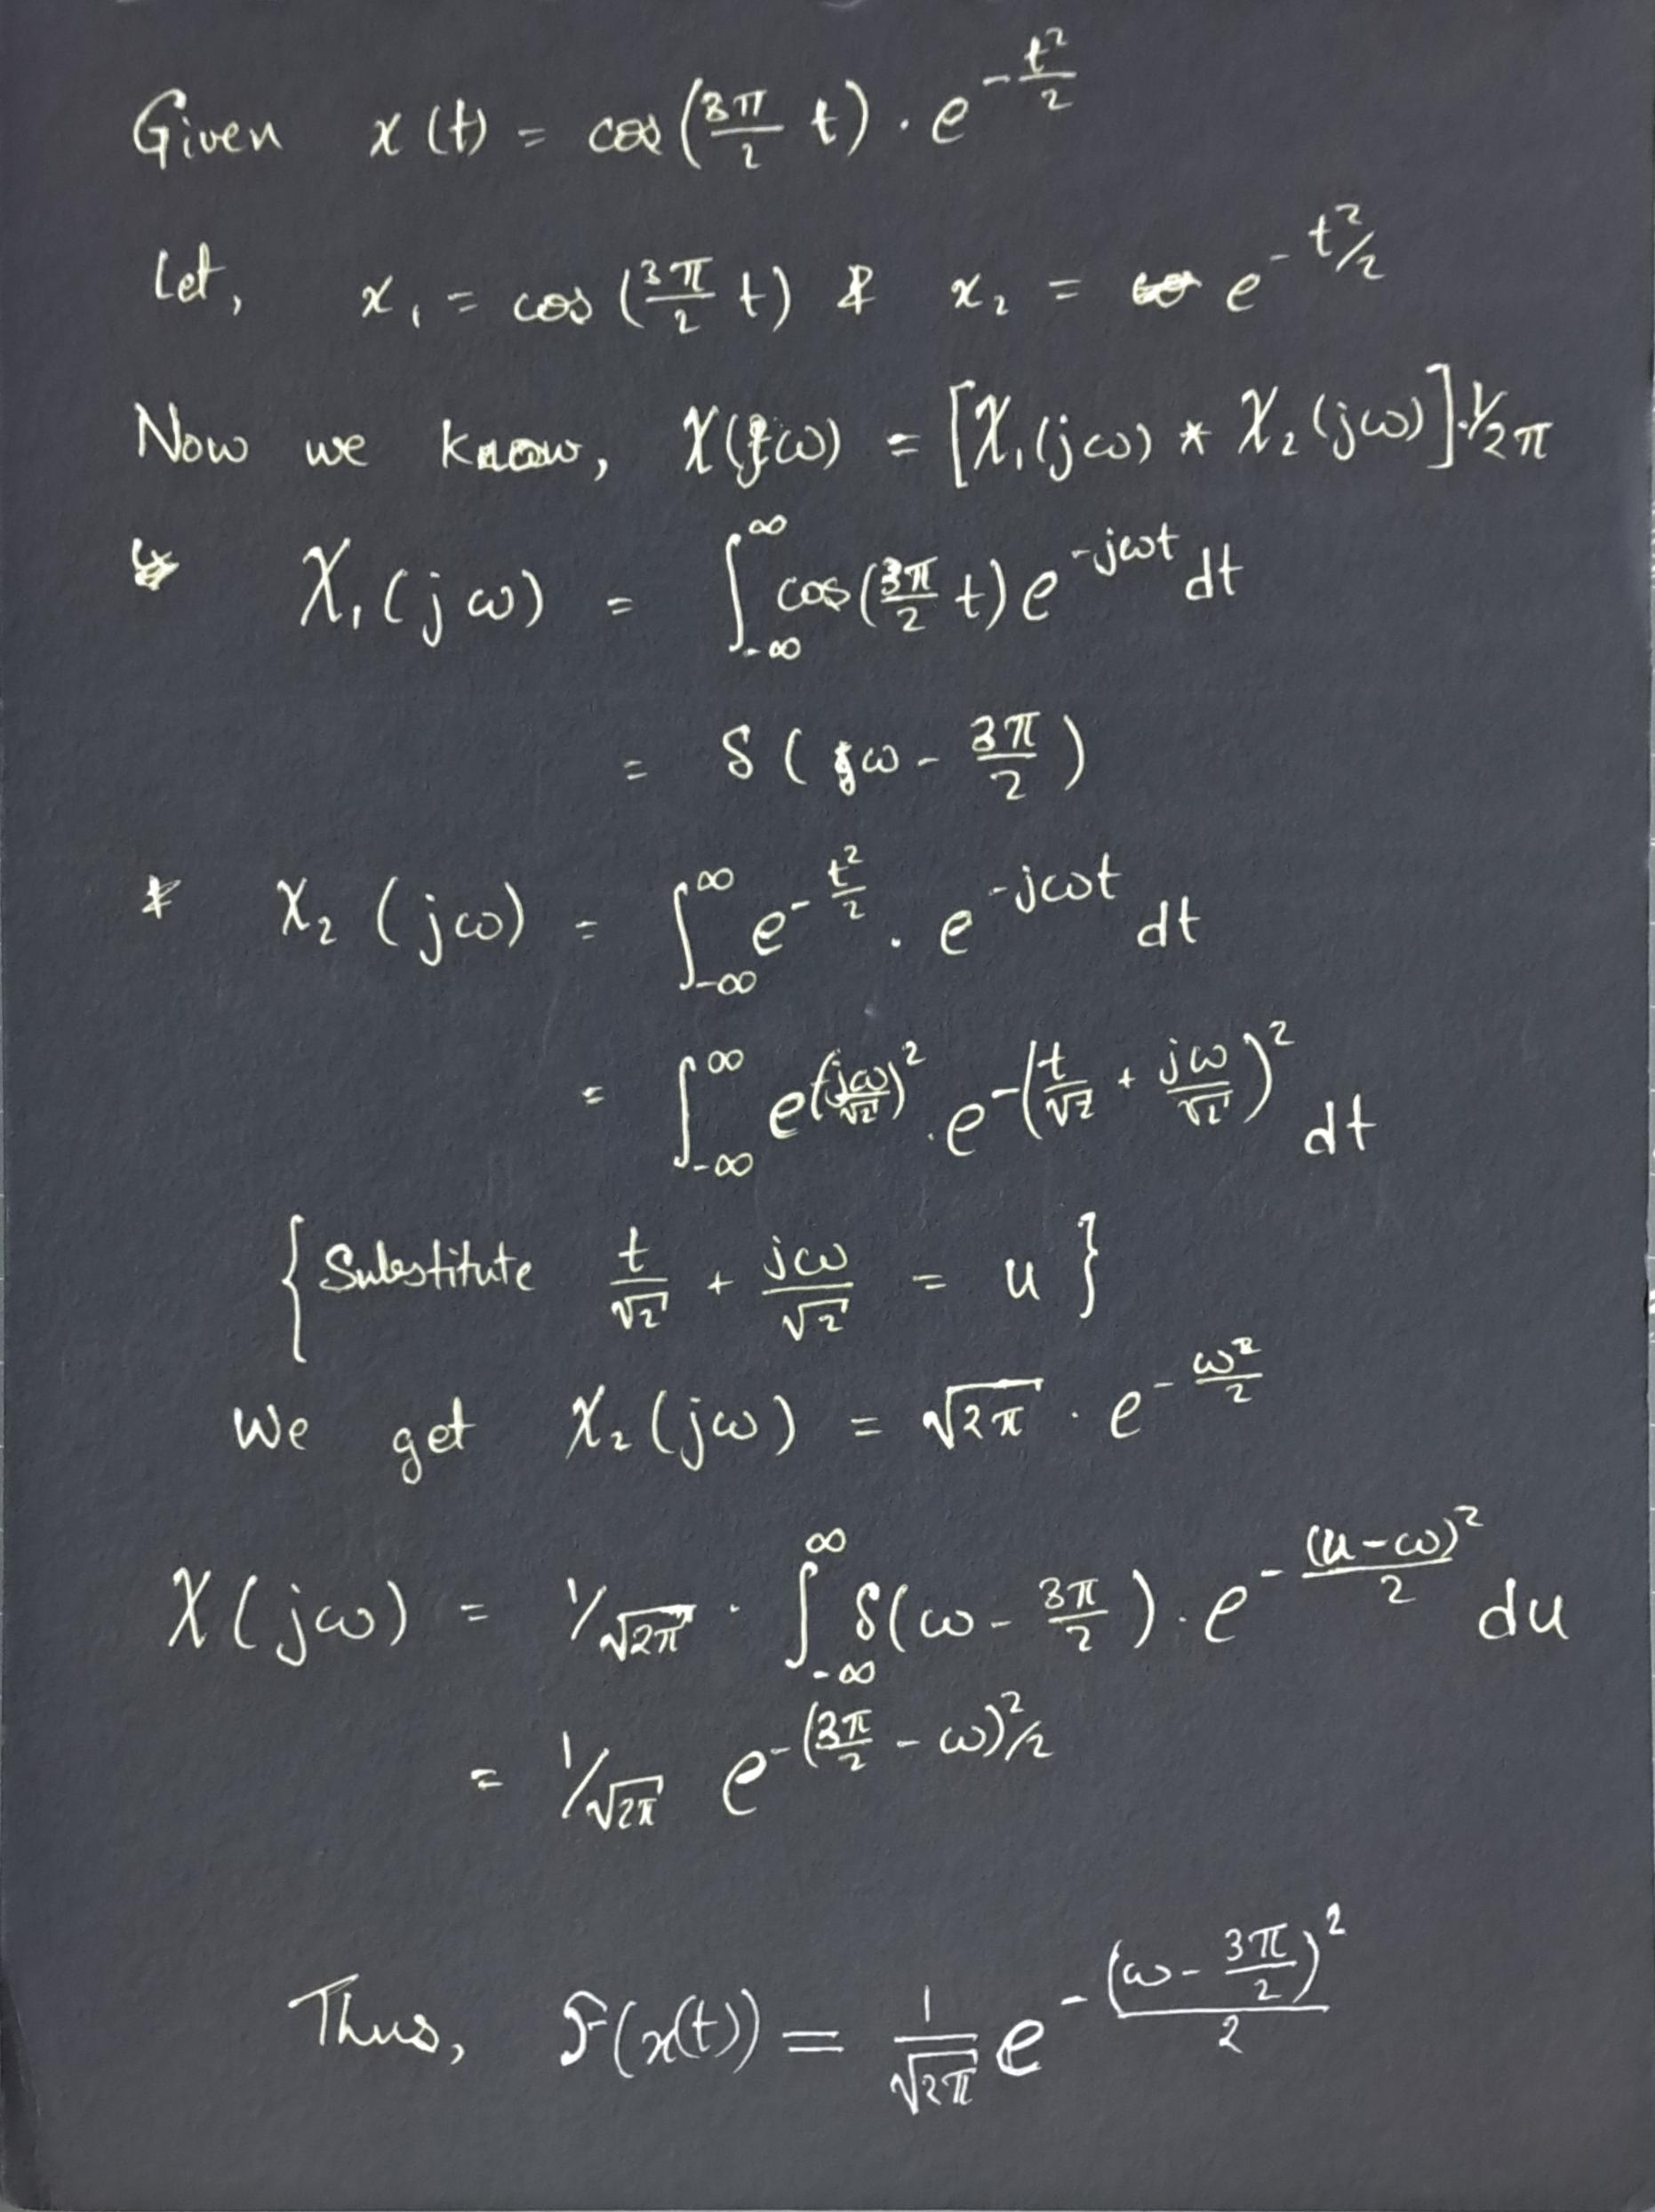
\includegraphics[width = .55\textwidth]{./imgs/2_solution.jpg}
\end{figure}

Final answer: $\frac{1}{\sqrt{2\pi}} \cdot e^{\frac{- \left(\omega - \frac{3\pi}{2}\right)^2}{2}}$


\pagebreak
\subsection*{MATLAB Code}

\[\] \vspace{-40px}

(b) Plot $\frac{1}{\sqrt{2\pi}} \cdot e^{\frac{- \left(\omega - \frac{3\pi}{2}\right)^2}{2}}$

\lstinputlisting[
    style=Matlab-Pyglike
]{matlab/22016_2b.m}

\[\] \vspace{-40px}

(c) Compare with the FT on sampled signal

\lstinputlisting[
    style=Matlab-Pyglike
]{matlab/22016_2c.m}


\subsection*{Output}

\begin{figure}[H]
    \centering
    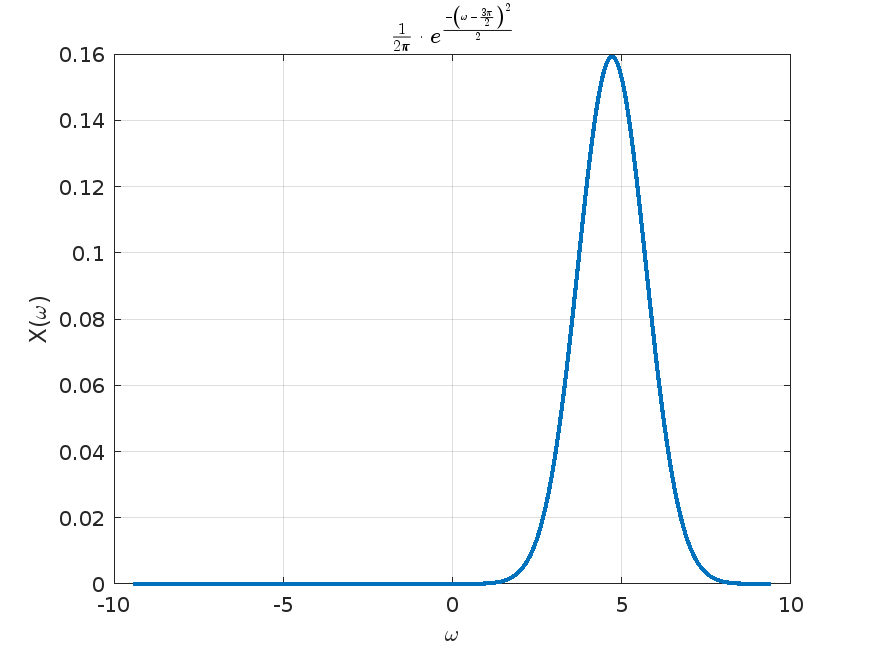
\includegraphics[width = .49\textwidth]{./imgs/2_plot_Xw.png}\hfill
    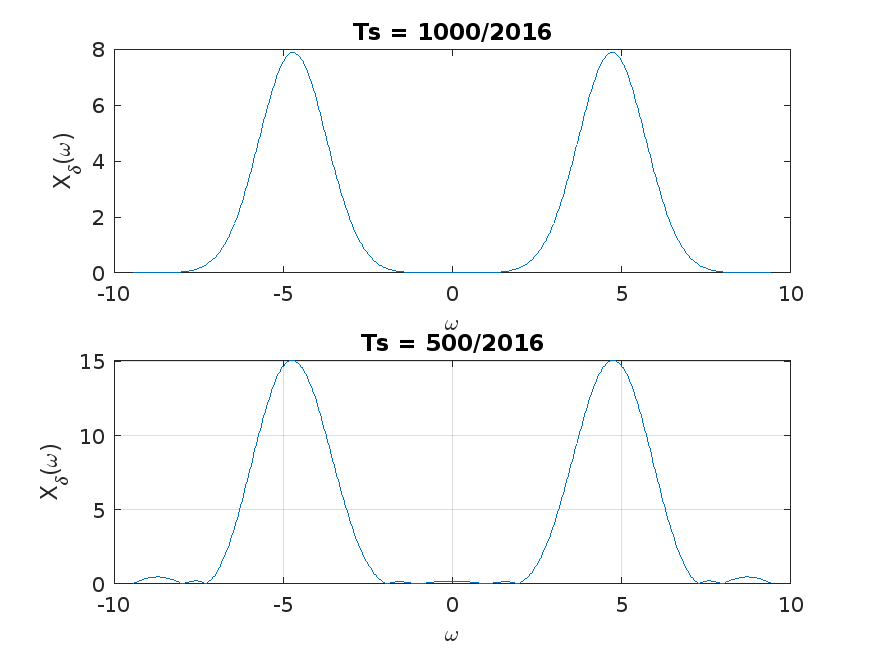
\includegraphics[width = .49\textwidth]{./imgs/2_plot_Xdelw.png}
    \caption {Plot of $X(j\omega)$ and $X_\delta(j\omega)$}
\end{figure}


\subsection*{Inference}

\begin{itemize}
    \item The plot of $X(j\omega)$ is a Gaussian function with a peak at $\omega = \frac{3\pi}{2}$.
    \item Looking at the graphs of $X_\delta(j\omega)$, one can very well approximate $X(j\omega)$ by sampling very few (in our case, 500) points and then computing the FT using summission formula.
    \item $X_\delta(j\omega)$ approximates $X(j\omega)$ very well at $T_s = \frac{2}{3\pi}$.
    \item There are multiple peaks at $X_\delta(j\omega)$ which is because, FT is periodic in case of sampled signals.
\end{itemize}